\subsection{Background}
\begin{frame}{Motivation}
    \begin{itemize}
        \item <1-2> Learners of the different/unshared prior knowledge (DK) condition had more \textcolor{purple}{difficulty coordinating their respective prior knowledge} compared to learners of the same/shared prior knowledge (SK) condition \cite{molinari2017learners}.
        
        \item <1-2> Participants with DK condition also \textcolor{purple}{focused their attention mainly in their own map and explored less their partner map} \cite{molinari2017learners}.

        \item <3->Limitation of our previous study
        \begin{itemize}
            \item <3-> In the experiment, partners were not chosen randomly.\\
            \textcolor{blue}{Whether or not group formation influences the results of collaboration?}
            \item <4>$\longrightarrow$ differentiate group based on their prior knowledge
        \end{itemize}
        
        
    \end{itemize}
\end{frame}
\begin{frame}{Research objectives}
\textcolor{blue}{Aim}:
    to investigate how individual differences in prior knowledge has potentially influenced collaborative-learning effectiveness and the students' perceptions toward the activities;
{
\setbeamercolor{block}{bg=red, fg=blue}
\begin{block}{Sub-research questions}
    \begin{enumerate}
    \item <1> What are the overall patterns of knowledge transfer from individual-to-group representation?
    \item <2> Does similarity of knowledge affect students' learning effectiveness in the two dimensions (i.e. interaction of individual members and group level), and, if so, to what extent?
    \item <3> Does similarity of knowledge affect the experiences of participants in the study, and, if so, to what extent?
\end{enumerate}
\end{block}
}


%% The study focuses on identifying the effectiveness from the end-products 
%% (collaborative maps), the patterns of map changes from individuals to groups, 
%% and the perceptions of the students while following the learning activities. 
\end{frame}

\subsection{Analysis methods}
\begin{frame}{Collected data and variables involved}
    \begin{figure}[tb]
     \begin{center}
      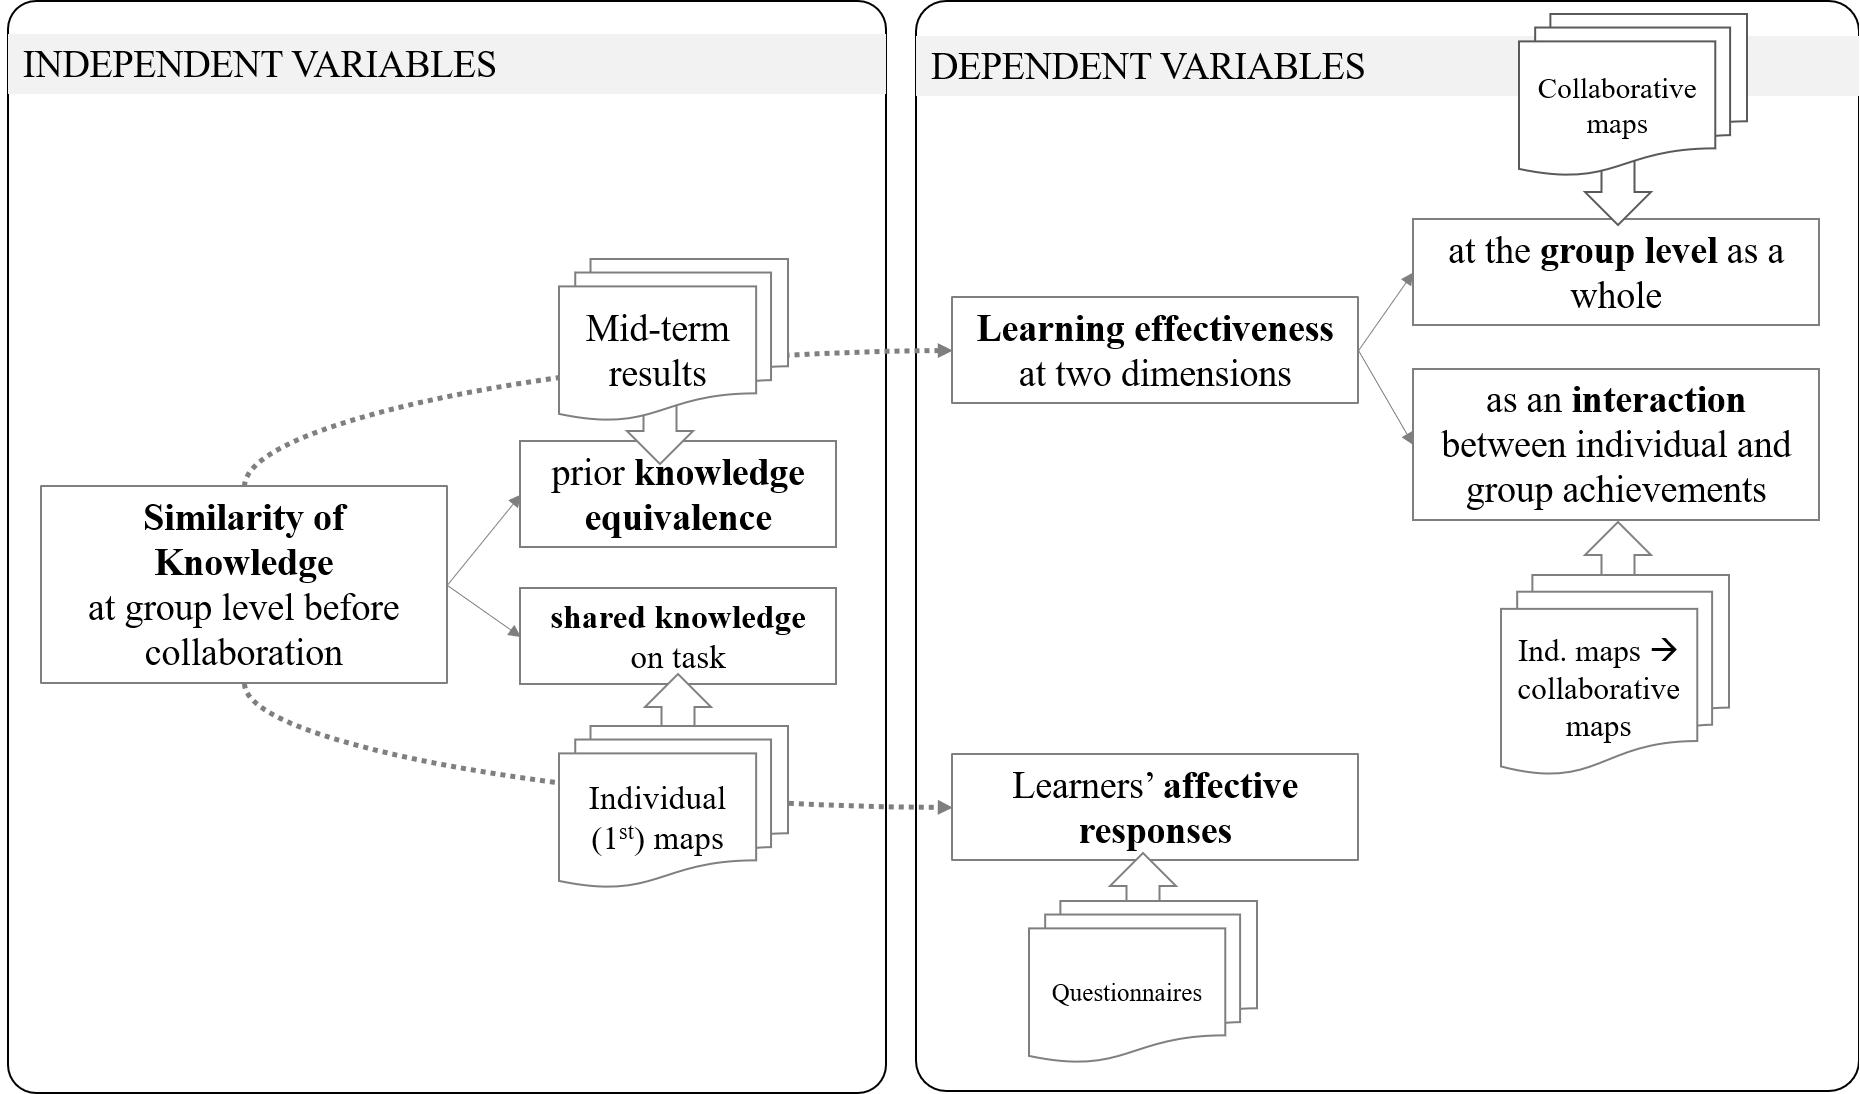
\includegraphics[width=100mm]{images/rqb_variables.pdf}
      \end{center}
      %\caption{Variables involved in this study}
      %\label{variables}  
\end{figure}
\end{frame}

\begin{frame}{Illustration of learning effectiveness analysis}
    \begin{figure}[tb]
     \begin{center}
      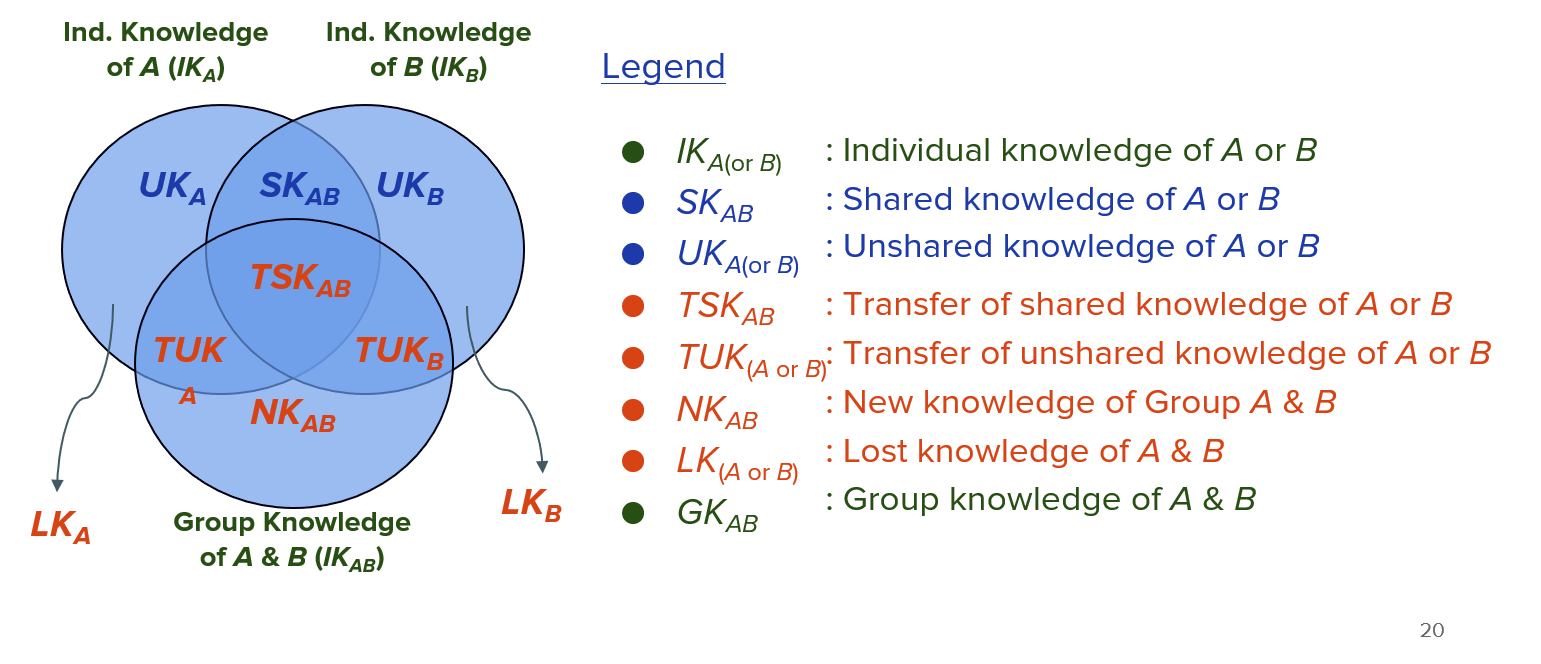
\includegraphics[width=110mm]{images/rqb_learning_effectiveness.png}
      \end{center}
      %\caption{}
      \label{learn-effective}  
    \end{figure}
\end{frame}

\subsection{Results \& discussions}
\begin{frame}{Overall pattern of knowledge transfer from individual-to-group representation}
    \begin{figure}[tb]
     \begin{center}
      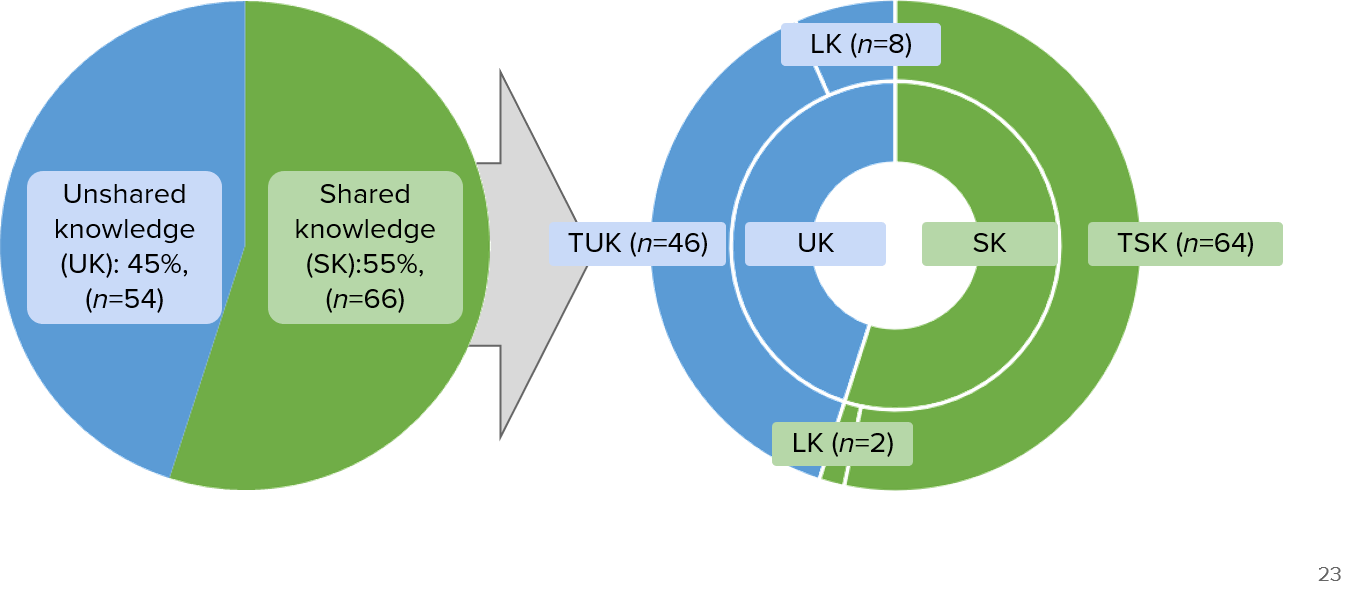
\includegraphics[width=100mm]{images/rqb_overall_transfer.png}
      \end{center}
      \caption{Distribution  of  shared  and  unshared  knowledge  in  individual maps \textcolor{blue}{prior to collaboration} (left) and distribution of individual \textcolor{blue}{knowledge transferred} to collaborative maps in all groups (right)}
      \label{rqb::result_dist}  
    \end{figure}
\end{frame}

\begin{frame}{Overall pattern of knowledge transfer from individual-to-group representation (cont'd)}
    Following the designated activities, learners are \textcolor{teal}{informed about their partner's understanding}, whether such knowledge is shared or unshared. Furthermore, they have a greater tendency to \textcolor{teal}{elaborate it into group knowledge}.
\end{frame}

\begin{frame}{Learning effectiveness at interaction level based on prior knowledge equivalence}
    \begin{figure}[tb]
     \begin{center}
      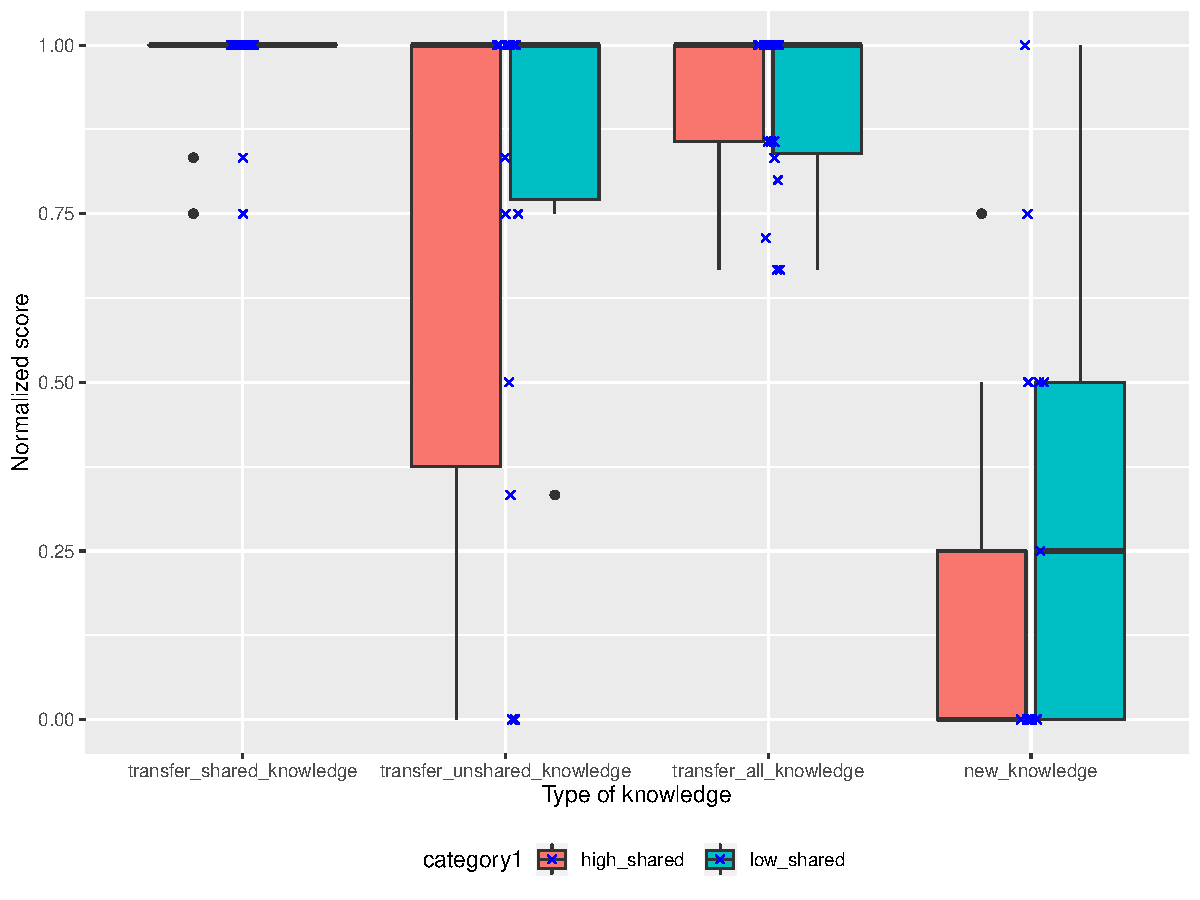
\includegraphics[width=90mm]{images/rqb_dist-shared-all-redraw.pdf}
      \end{center}
      \caption{Distribution of knowledge transfer and new knowledge in high-and  low-prior-knowledge-equivalence  groups}
      \label{rqb::dist_equival}  
    \end{figure}

\end{frame}
    
\begin{frame}{Learning effectiveness at interaction level based on shared knowledge on task}
    \begin{figure}[tb]
     \begin{center}
      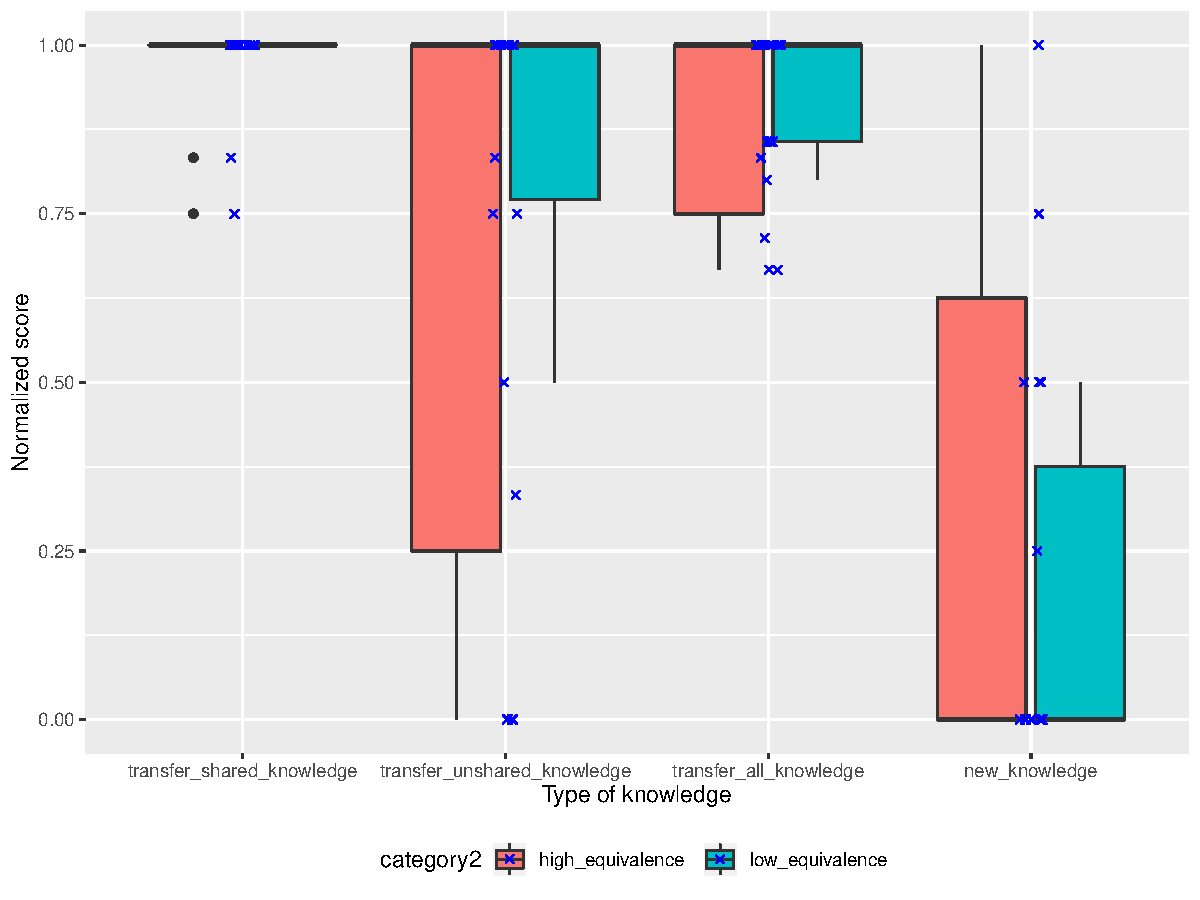
\includegraphics[width=90mm]{images/rqb_dist-equivalence-all-redraw.pdf}
      \end{center}
      \caption{Distribution of knowledge transfer and new knowledge in high-and low-shared-knowledge groups}
      \label{rqb::dist_shared}  
    \end{figure}
    
\end{frame}



\begin{frame}{Learning effectiveness at interaction level (i.e. knowledge transfer and new knowledge)}
    \begin{enumerate}
        \item <1> The amount of shared and unshared knowledge transfer from all groups in all conditions remained at \textcolor{teal}{the same level (similar median values)}, with \textcolor{purple}{differences in score distribution}.
        \item <2-3> Based on the knowledge-equivalence scores, the group creativity scores in both conditions show \textcolor{teal}{similar median values}, though the \textcolor{purple}{distribution is different}. 
        \item <3> The low-shared-knowledge groups have \textcolor{teal}{higher} new knowledge scores than high-shared-knowledge groups.
    \end{enumerate}
\end{frame}

\begin{frame}{Learning effectiveness at group level}
    
    \begin{figure}[tb]
     \begin{center}
      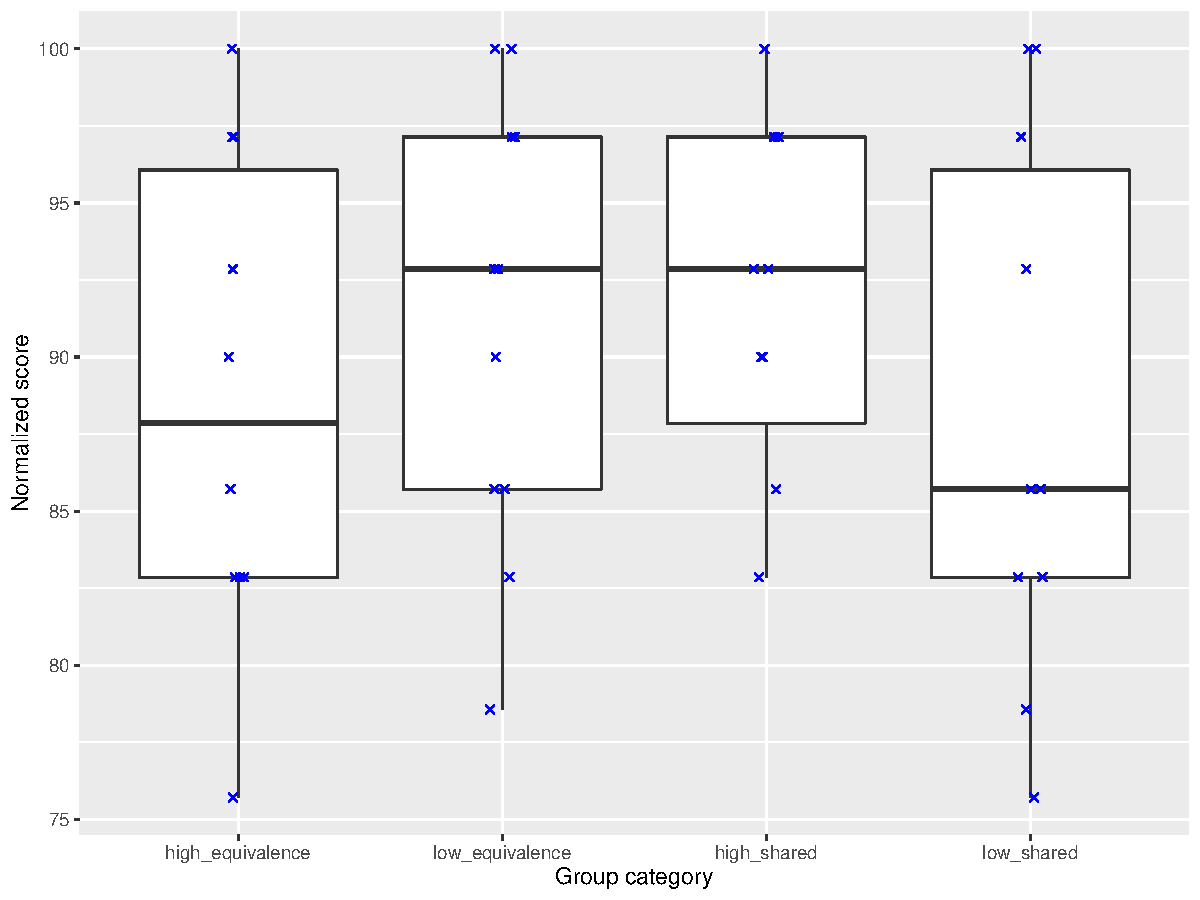
\includegraphics[width=90mm]{images/rqb_group-map-redraw.pdf}
      \end{center}
      %\caption{Collaborative map scores differentiated by prior-knowledge equivalence and shared knowledge about the task}
      \label{rqb::group-map}  
    \end{figure}
\end{frame}



\begin{frame}{Learning effectiveness at group level (cont'd)}

    {\small According to Welch's t-test, the group achievement scores \textcolor{blue}{do not differ significantly} between low- and high-knowledge-equivalence conditions, $t(18.3) = -0.74, p = .47, d = 0.32$, 95\% CI [-9.43  4.53], or between low- and high-shared-knowledge conditions, $t(15.6) = 1.07, p = .30, d = 0.48$, 95\% CI [-3.50, 10.6]}
    %, though there is \textcolor{blue}{dissimilarity of distribution among them}.
\end{frame}


\begin{frame}{Learners' affective responses across  different  shared-knowledge scores}
    \begin{figure}[tb]
     \begin{center}
      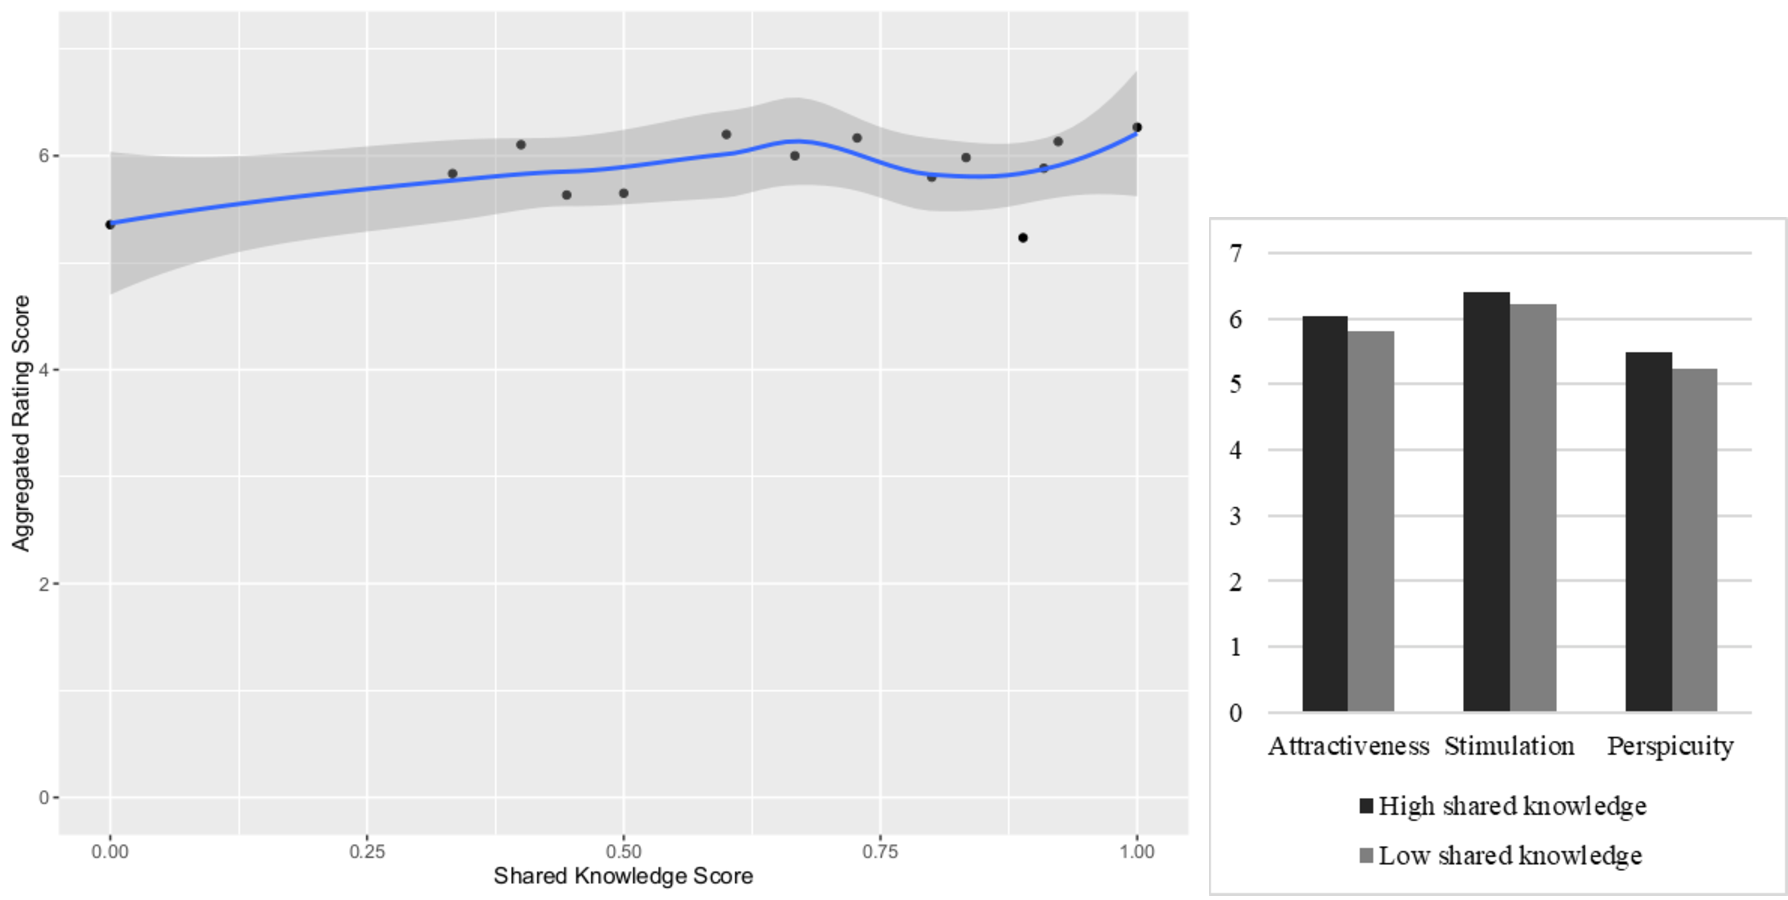
\includegraphics[width=80mm]{images/rqb_affective-response-redraw.pdf}
      \end{center}
      %\caption{Distribution  of  affective  responses  across  different  shared-knowledge scores}
      \label{rqb::affective}  
    \end{figure}
    
    A Kruskal–Wallis rank-sum test indicates that there is a significant difference between the homogeneous and heterogeneous group regarding their affective responses \textcolor{blue}{($H(13) = 56.8, p < .001$)}. 
    %However, these differences, though significant, are rather small.

\end{frame}

\begin{frame}{Open-ended survey results}
Some participants in both homogeneous and
heterogeneous groups reported \textcolor{purple}{comparable on-task 
difficulties concerning dissimilarities of ideas or 
opinions}, i.e.:
{\small
\begin{itemize}
    \item “Difficult to read when the number of visualized differences is too many ($n = 6$)”
    \item “It was hard to read or understand the difference map ($n = 2$)”
    \item "It was difficult to integrate different opinions in order to reach a (group) consensus or determine which one is the correct representation ($n = 5$)"
    \item “The use of ambiguous links makes it hard to select the most suitable relation between two concepts ($n = 1$)”
\end{itemize} 
}
\end{frame}

\begin{frame}{Key findings}
    \textcolor{blue}{Research aim [B]}: to investigate how individual differences in prior knowledge has potentially influenced collaborative-learning effectiveness and the students’ perceptions toward the activities
    
    \begin{block}{}
        \begin{enumerate}
            %\item <+-> Following the designated activities, learners are \textcolor{teal}{informed about their partner's understanding}, whether such knowledge is shared or unshared. Furthermore, they have a greater tendency to \textcolor{teal}{elaborate it into group knowledge}.
            \item <+-> Groups with high and low similarity of knowledge \textcolor{teal}{achieved similar learning effectiveness} at the level of interaction between individuals and group as whole.
            %\item <+-> The amount of \textcolor{blue}{joint knowledge} within the group may possibly affect group outcomes.
            \item <+-> Different opinions or perspectives on the task itself slightly \textcolor{purple}{influenced the learners’ overall experiences} within a collaborative environment. 
        \end{enumerate}
    \end{block}
\end{frame}